\documentclass[10pt, letterpaper]{article}

\usepackage{amssymb,amsmath,amsfonts,eurosym,geometry,ulem,graphicx,caption,color,setspace,sectsty,comment,footmisc,caption,natbib,pdflscape,subfigure,array,hyperref}
\usepackage{xcolor}
\usepackage{mathptmx}
\usepackage{listings}
\lstset{language=Matlab}
\hypersetup{
    colorlinks,
    linkcolor={red!50!black},
    citecolor={blue!50!black},
    urlcolor={blue!80!black}
}
\normalem
\usepackage[flushleft]{threeparttable}
    
\onehalfspacing
\newtheorem{theorem}{Theorem}
\newtheorem{corollary}[theorem]{Corollary}
\newtheorem{proposition}{Proposition}
\newenvironment{proof}[1][Proof]{\noindent\textbf{#1.} }{\ \rule{0.5em}{0.5em}}

\newtheorem{hyp}{Hypothesis}
\newtheorem{subhyp}{Hypothesis}[hyp]
\newtheorem{asu}{Assumption}
\renewcommand{\thesubhyp}{\thehyp\alph{subhyp}}

\newcommand{\red}[1]{{\color{red} #1}}
\newcommand{\blue}[1]{{\color{blue} #1}}

\newcolumntype{L}[1]{>{\raggedright\let\newline\\arraybackslash\hspace{0pt}}m{#1}}
\newcolumntype{C}[1]{>{\centering\let\newline\\arraybackslash\hspace{0pt}}m{#1}}
\newcolumntype{R}[1]{>{\raggedleft\let\newline\\arraybackslash\hspace{0pt}}m{#1}}

\geometry{left=1.0in,right=1.0in,top=1.0in,bottom=1.0in}

\begin{document}

\title{Homework 7 (Homework 2 for Spring Semester):\\ ECON512}
\author{Joonkyo Hong}
\date{}
\maketitle
\smallskip

\noindent Q1. For this question, I completely follow the guideline in the problem set. For this exercise, I start with the following initial guesses.

\begin{align*}
   \bold{P} & = [ c(\omega) , c(\omega) , c(\omega)  , \hdots , c(\omega)] \in \mathbb{R}^{L \times L} \\
   \bold{V} & = \bold{0}_{L \times L}.
\end{align*}
With this guess, I achieve a equilibrium in about 80 seconds with 170 iterations. Figure 1 is displaying the value and policy functions.\\

\noindent Q2. Let $( \hat{p}_{1}(\omega), \hat{p}_{2}(\omega) )$ be a equilibrium strategy profile given state $\omega$. Let $\omega^{'}$ be a future state. Then in this equilibrium, the transition matrix of state $\omega$ can be computed by following:
\begin{align*}
 \pi(\omega^{'}|\omega) = & D_{0}(\hat{p}_{1}(\omega), \hat{p}_{2}(\omega)) P(\omega_{1}^{'}|\omega_{1},q_{1}=0) P(\omega_{2}^{'}|\omega_{2},q_{2}=0)  \\
                          & + D_{1}(\hat{p}_{1}(\omega), \hat{p}_{2}(\omega)) P(\omega_{1}^{'}|\omega_{1},q_{1}=1) P(\omega_{2}^{'}|\omega_{2},q_{2}=0) \\
                          & + D_{2}(\hat{p}_{1}(\omega), \hat{p}_{2}(\omega)) P(\omega_{1}^{'}|\omega_{1},q_{1}=0) P(\omega_{2}^{'}|\omega_{2},q_{2}=1) 
\end{align*}

Following the above formula, I construct $L^{2} \times L^{2}$ matrix $\Pi$. I start with $1 \times L^{2}$ vector $p=(1,0,0, \hdots, 0)$, and compute the distribution of the state through
\begin{align*}
    p^{k} = p\Pi^{k},
\end{align*}
where $k=10,20,30$. With a proper reshaping process, I could plot the distribution on $\{1,2,\hdots,L \} \times \{1,2,\hdots,L\}$. Figure 2 is displaying the distributions of the state after 10, 20, and 30 periods later, respectively. \\

\noindent Q3. Upon getting the transition matrix $\Pi$, it is straightforward to obtain the stationary distribution. Start with any initial state vector $\nu^{1}$, I could compute the stationary distribution as $\Pi$ is ergodic Markov transition matrix. The stationary distribution emerging from the equilibrium computed in Q1 is displayed in Figure 3.



\begin{figure}
\centering
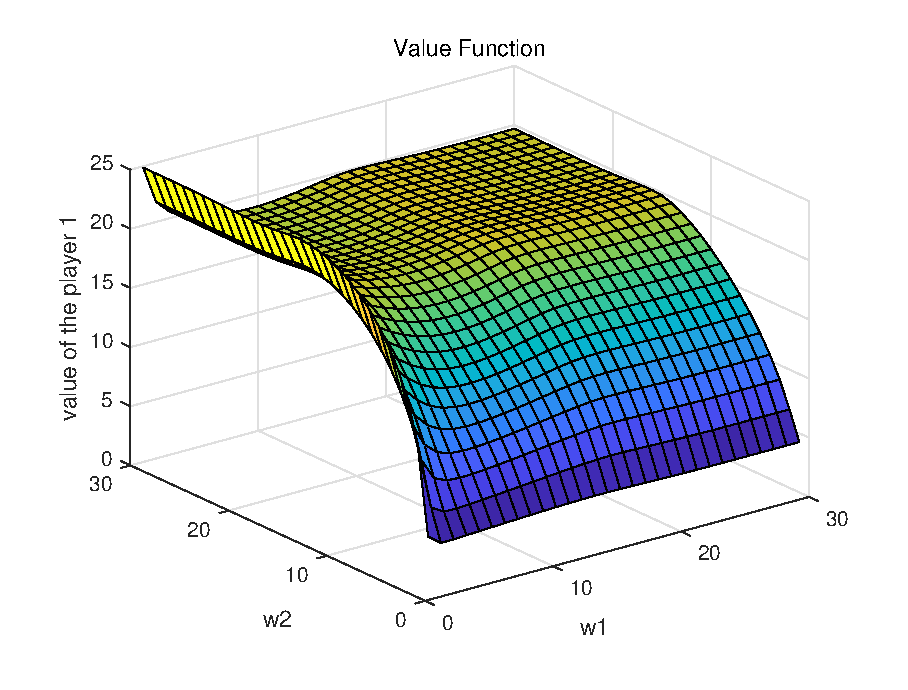
\includegraphics[width=0.5\textwidth]{value.eps}\\
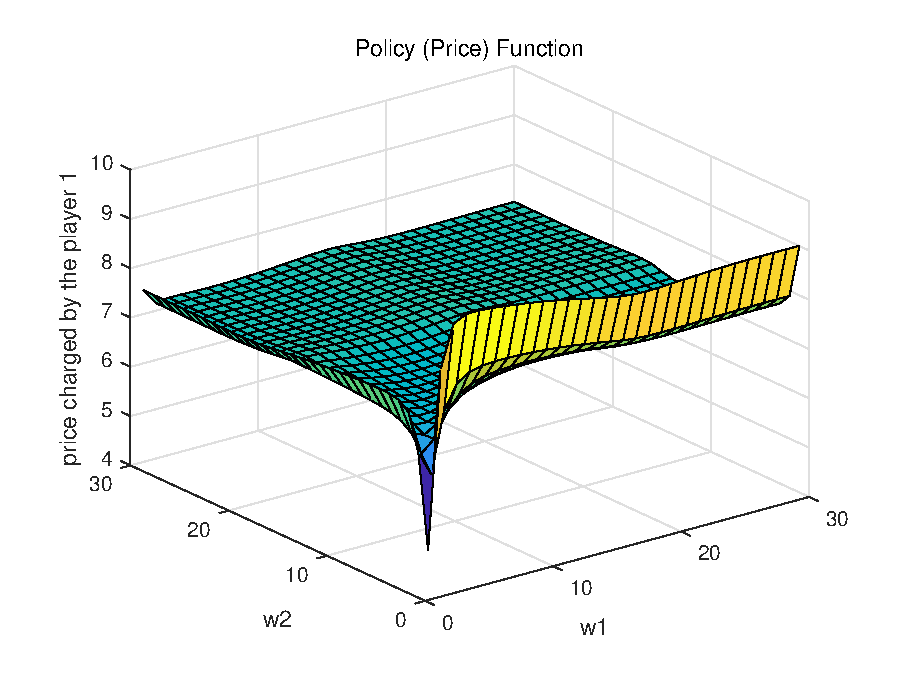
\includegraphics[width=0.5\textwidth]{policy.eps}
\caption{Value and Policy Functions}
\end{figure}


\begin{figure}
\centering
\includegraphics[width=0.5\textwidth]{10period.eps}\\
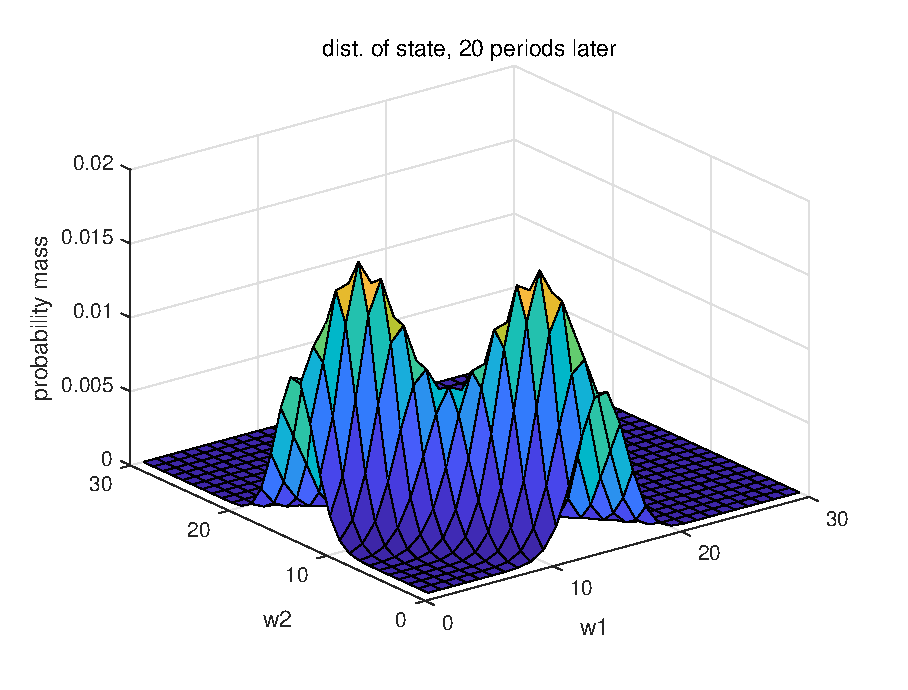
\includegraphics[width=0.5\textwidth]{20period.eps}\\
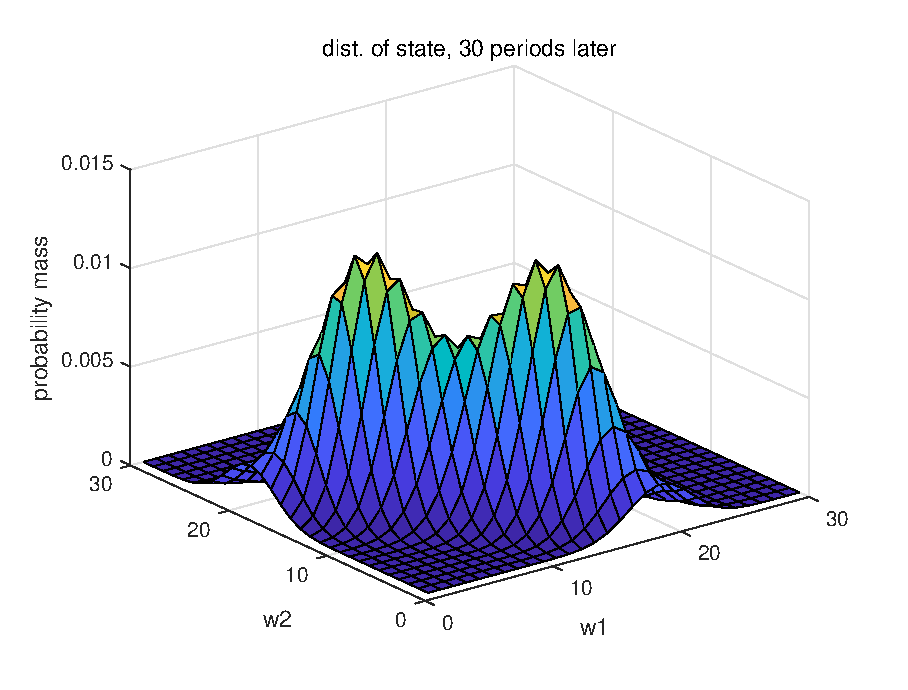
\includegraphics[width=0.5\textwidth]{30period.eps}
\caption{Evolution of Distribution of State}
\end{figure}


\begin{figure}
\centering
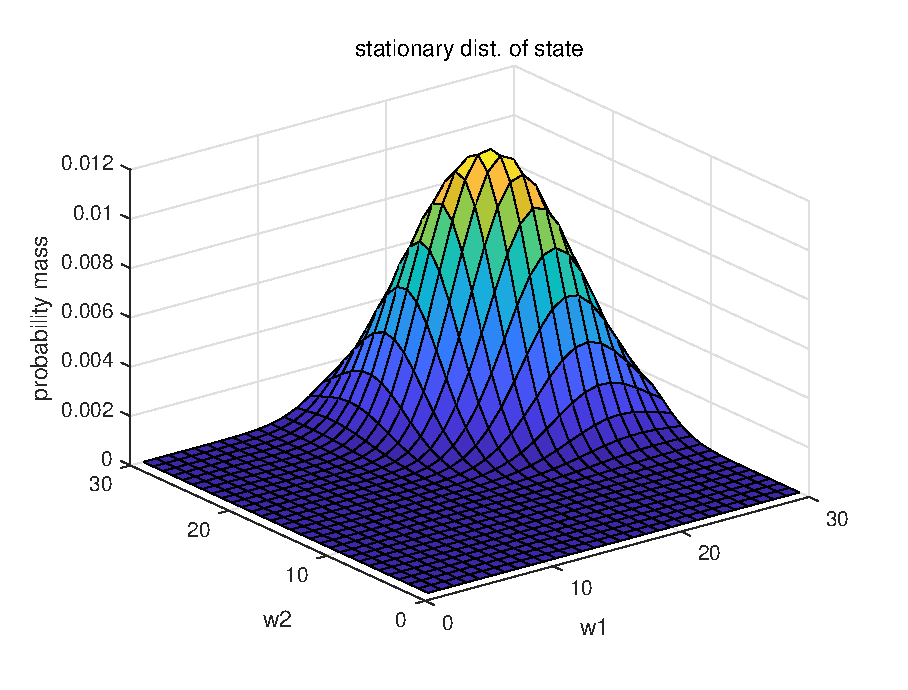
\includegraphics[width=0.8\textwidth]{stationary.eps}
\caption{Stationary Distribution of State}
\end{figure}


\clearpage

\begin{verbatim}
% Code for HW2 in Spring (HW7) ECON512
% Written by Joonkyo Hong
% Build upon codes contained in code_QLD in ECON512 lecture
% Feb 16, 2019

clear;

%% Question 1. Solve for the equilbrium through policy and value function iteration

run prmtr.m
global L eta kappa l nu delta betta lambda eps cost trans0 trans1
iter=0;
diff=10;
maxiter = 5000;

P0=repmat(cost,1,L);                      % competitive price
V0=zeros(L,L);

 tic
 while diff > eps && iter < maxiter
   
     % Policy function updating
           
           g = @(x) P_FOC(V0,x);
           P1 = fsolve(g,P0);
           
      % With updated P1, update the value function
      
           V1 = updateV(V0, P1, P0);
           
      % difference is
      
           diff = max(max(max(abs((V1-V0)./(1+V1)))),  max(max(abs((P1-P0)./(1+P1))))); 
           
      % Dampening
         
           V0 = (1-lambda)*V0 + lambda*V1;
           P0 = (1-lambda)*P0 + lambda*P1;
           
      % Go Next Iteration
      
       iter = iter+1;
       
       clc;
       disp('current iteration');
       disp(num2str(iter));
       disp('current difference');
       disp(num2str(diff));
       
       
 end   
 toc
 
 
 figure(1)
 surf((1:1:L),(1:1:L),V1);
 title("Value Function");
 
 figure(2)
 surf((1:1:L),(1:1:L),P1);
 title("Policy (Price) Function"); 
 
 
 %% Question 2. Compute the distribution of the state as time evolves
 
    % D0, D1, D2 in the equilibrium computed in Section 1.
    [D0eqm, D1eqm, D2eqm] = computeD(P1,P1');
    
    D0state = repmat(reshape(D0eqm',L*L,1),1,L*L);
    D1state = repmat(reshape(D1eqm',L*L,1),1,L*L);
    D2state = repmat(reshape(D2eqm',L*L,1),1,L*L); 
    
    % Conditional on each learning status, compute the transition matrix
    State0 = kron(trans0, trans0);
    State1 = kron(trans1, trans0);
    State2 = kron(trans0, trans1);
    
    % Finally the transition martrix is
    Pi = D0state.*State0 + D1state.*State1 + D2state.*State2;
    Pi = Pi./repmat(sum(Pi,2),1,L*L);     % To rule out the numerical noises making the sum exceed one
    
    % Compute the distribution of states after 10, 20, and 30 periods
    
    Pi10 = Pi^10;
    Pi20 = Pi^20;
    Pi30 = Pi^30;
    start = [1 zeros(1,899)];
   
    state10 = start*Pi10;
    state10 = reshape(state10,L,L);    % distribution of states, 10 periods later, L by L matrix
    state20 = start*Pi20;
    state20 = reshape(state20,L,L);    % distribution of states, 20 periods later, L by L matrix
    state30 = start*Pi30;
    state30 = reshape(state30,L,L);    % distribution of states, 30 periods later, L by L matrix
    
    figure(3)
    surf(1:1:L,1:1:L,state10);
    xlabel('w1');
    ylabel('w2');
    zlabel('probability mass');
    title('dist. of state, 10 periods later');
    
    figure(4)
    surf(1:1:L,1:1:L,state20);
    xlabel('w1');
    ylabel('w2');
    zlabel('probability mass');    
    title('dist. of state, 20 periods later');

    figure(5)
    surf(1:1:L,1:1:L,state30);
    xlabel('w1');
    ylabel('w2');
    zlabel('probability mass'); 
    title('dist. of state, 30 periods later');

    
%% Question 3. Compute the stationary distribution of the state

   start = [1 zeros(1,899)];

         diff=1;

         while diff>10e-16
               update=start*Pi;
               diff=norm(update-start)/norm(start);
               start=update;
         end
     
   stationary = reshape(update,L,L);
   
    figure(6)
    surf(1:1:L,1:1:L,stationary);
    xlabel('w1');
    ylabel('w2');
    zlabel('probability mass');
    title('stationary dist. of state');

\end{verbatim}
                     

\end{document}